\section{Hyperparameters and Search Space}
\label{app:hp}

All values below are the configuration files used for every reported run.

\begin{table}[h]
\centering\small
\begin{tabular}{@{}llr@{}}
\toprule
Symbol & Role & Default \\
\midrule
$w_{\text{ans}}$ & answer F1 (terminal) & 1.0 \\
$w_{\text{hop}}$ & on-gold, order-consistent hop & 0.2 \\
$w_{\text{red}}$ & revisited entity & 0.1 \\
$w_{\text{schema}}$ & schema-inconsistent last cell & 0.05 \\
$w_{\text{step}}$ & per selected entity & 0.02 \\
$w_{\text{stop}}$ & stop after all gold seen & 0 \\
$w_{\text{path}}$ & trace-level path F1 (B2b only) & 0.2 \\
\bottomrule
\end{tabular}
\caption{Reward weights. A1 and B2a zero all hop terms and the schema term; B2b adds $w_{\text{path}}$ at the end of the trace.}
\label{tab:reward-weights}
\end{table}

\begin{table}[h]
\centering\small
\begin{tabular}{@{}p{0.62\columnwidth}p{0.3\columnwidth}@{}}
\toprule
Parameter & Value \\
\midrule
Candidates $K$ / column top-$k$ / max hops $H$ & 32 / 8 / 4 \\
BM25 weight at hop 0 & 0.5 \\
Encoder (frozen) & bge-small-en-v1.5 \\
Policy hidden size & 256 \\
PPO $\gamma$, $\lambda$, clip $\epsilon$ & 1.0, 0.95, 0.2 \\
Value coef., entropy coef. (linear decay) & 0.5, 0.01 \\
Epochs, minibatch, grad clip & 4, 256, 0.5 \\
Learning rate (Adam) & $3\times10^{-4}$ \\
Rollout batch (PPO) & 64 trajectories \\
GRPO group size, questions per update & 8, 8 \\
Budget (RL) & 48{,}000 trajectories \\
Dev evaluation & every 50 updates, 300 questions \\
Cache of environments & 512 \\
\bottomrule
\end{tabular}
\caption{Environment and RL hyperparameters.}
\label{tab:rl-hp}
\end{table}

\begin{table}[h]
\centering\small
\begin{tabular}{@{}p{0.2\columnwidth}p{0.72\columnwidth}@{}}
\toprule
Component & Setting \\
\midrule
Answer head & flan-t5-small; 3 epochs, lr $3\times10^{-4}$, batch 16 \\
 & distractors: $p=0.3$, 1--2 entities; max 512 / 32 tokens \\
B1 (SFT) & 48{,}000 examples, batch 16, lr $3\times10^{-4}$ \\
 & max 512 tokens, 200 passage characters per link \\
B3 (soft) & 48{,}000 examples, batch 16, lr $10^{-3}$, wd 0.01 \\
 & hidden 256, dropout 0.1, top-3 \\
\bottomrule
\end{tabular}
\caption{Answer-head, B1 and B3 hyperparameters.}
\label{tab:other-hp}
\end{table}

\paragraph{Search space.}
Each trained method receives three trials on dev with seed 0 (default first): RL methods (H1, B2a, B2b): default, $\text{lr}=10^{-3}$, entropy coefficient $0.03$; B3: lr $\in\{10^{-3},3\times10^{-4},3\times10^{-3}\}$; B1: lr $\in\{3\times10^{-4},10^{-4},10^{-3}\}$.
The setting with the highest full-dev EM (ties by F1) is selected, non-selected trials are archived and final runs use seeds 0, 1 and 2.
Ablations A1--A4 inherit the setting chosen for H1.
Reward weights are not tuned.
Table~\ref{tab:study} lists every trial and its full-dev EM.
\begin{table}[t]
\centering\small
\resizebox{\columnwidth}{!}{\begin{tabular}{lllll}
\toprule
method & trial & setting & dev EM & chosen \\
\midrule
B1 SFT & t0 & default & 26.3 &  \\
B2a GRPO & t0 & default & 10.1 &  \\
B2a GRPO & t1 & ppo.lr\_head=1.0e-3 & 10.5 &  \\
B2a GRPO & t2 & ppo.entropy\_coef=0.03 & 11.7 &  \\
B2b GRPO+path & t0 & default & 7.4 &  \\
B2b GRPO+path & t1 & ppo.lr\_head=1.0e-3 & 7.0 &  \\
B3 soft & t0 & default & 13.9 &  \\
H1 Hop-PPO & t0 & default & 11.4 &  \\
H1 Hop-PPO & t1 & ppo.lr\_head=1.0e-3 & 8.1 &  \\
H1 Hop-PPO & t2 & ppo.entropy\_coef=0.03 & 9.9 &  \\
\bottomrule
\end{tabular}
}
\caption{Tuning trials (dev, seed 0) and the selected setting per method.}
\label{tab:study}
\end{table}

\section{Design Changes Made During Development}
\label{app:changes}

The following design decisions were made on the dev split, before any test or OOD evaluation, and were applied to every compared method.
\paragraph{Candidate features.}
A first Hop-PPO run (seed 0) reached a low dev EM, and diagnostics on 300 dev questions showed that behaviour cloning on gold paths could not recover the first hop because the policy saw only embeddings, whereas the gold anchor is largely lexical.
We added four per-candidate features (cosine, normalized BM25, question-token overlap with the entity, overlap with the header) to the policy of H1, A1--A4, B2a and B2b and to the scorer of B3.
Runs made before this change are excluded from all results.
\paragraph{Row evidence.}
The answer head now reads each selected cell as its whole row, with passages visible only if selected; the head was retrained accordingly.
The change was applied to every path method and to M0, and was chosen on dev EM of a single H1 run against the entity-only rendering.
\paragraph{Tuning budget.}
Three instead of six trials per method (Appendix~\ref{app:hp}), equal for all methods, because of the time and compute available.
\paragraph{Review fix.}
During review we found and fixed an exploit in which revisiting a gold entity re-earned the hop reward; revisits now earn no hop reward.

\section{Data Statistics}
\label{app:data}

Table~\ref{tab:splits} gives split sizes.
Gold-path coverage is \GoldCovTrain\% on train and every path is heuristic; the share of heuristic paths whose last entity text contains the gold answer string is a lower bound on label correctness.
Table~\ref{tab:datastats} gives per-split statistics; first-gold-entity recall of the hop-0 candidates ($K=32$) is \RecallKDev\% on dev.
\begin{table}[t]
\centering\small
\resizebox{\columnwidth}{!}{\begin{tabular}{llllllll}
\toprule
split & n & n\_tables & frac\_heuristic & path\_len\_mean & ans\_type\_passage & rows\_mean & cols\_mean \\
\midrule
train & 3000 & 2564 & 0.9907 & 2.046 & 1683 & 15.86 & 4.55 \\
dev & 1000 & 844 & 0.988 & 2.071 & 589 & 15.62 & 4.57 \\
test & 2045 & 1787 & 0.9736 & 2.113 & 1220 & 15.67 & 4.54 \\
ood\_test & 569 & 498 & 0.9613 & 2.13 & 314 & 16.5 & 4.19 \\
ood\_dev & 500 & 429 & 0.99 & 2.075 & 264 & 16.12 & 4.33 \\
\bottomrule
\end{tabular}
}
\caption{Per-split statistics: questions, distinct tables, share with a heuristic gold path, mean gold-path length, passage answers, mean rows and columns.}
\label{tab:datastats}
\end{table}

\section{Additional Figures}
\label{app:figs}

\begin{figure}[t]
\centering
\figfile{F10_reward_components}{width=\columnwidth}
\caption{Reward components of \hop\ (seed 0) per training update, 25-update moving average: hop reward, redundancy penalty, schema penalty, step cost and terminal answer reward (reward-hacking check).}
\label{fig:reward}
\end{figure}
\begin{figure}[t]
\centering
\figfile{F7_hop_counts}{width=\columnwidth}
\caption{Distribution of the number of selected hops per method.}
\end{figure}
\begin{figure}[t]
\centering
\figfile{F5_ablations}{width=\columnwidth}
\caption{Ablation results with intervals (graphical version of Table~\ref{tab:ablations}).}
\end{figure}
\IfFileExists{../results/figures/F6_id_vs_ood.pdf}{\begin{figure}[t]
\centering
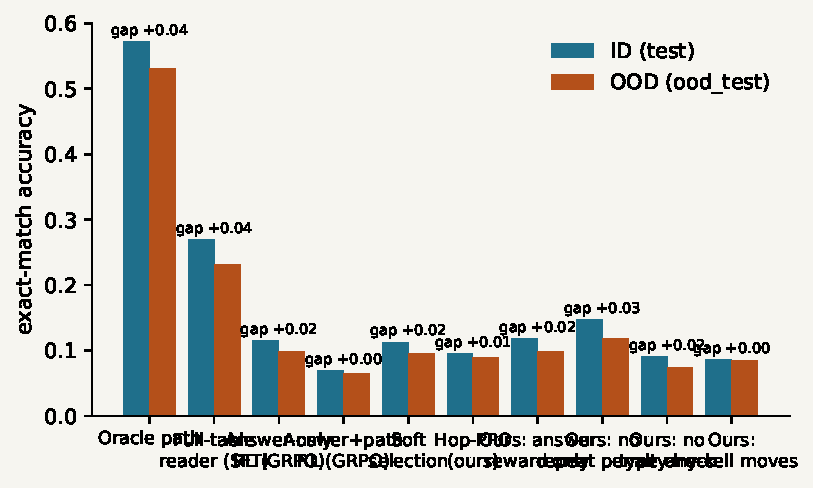
\includegraphics[width=\columnwidth]{../results/figures/F6_id_vs_ood.pdf}
\caption{ID versus OOD EM per method with gap.}
\end{figure}}{}

\section{Reproducibility}
\label{app:repro}

Every run records its seed, configuration, device and code version, per-update training logs and per-question predictions; splits are fixed by question ids and checksums, and an automatic check confirms that no table is shared between splits before evaluation.
All tables and figures are generated from the run logs by scripts, never by hand.
All runs use one pinned software environment.
The full pipeline takes about 12--15 hours on our laptop.

\section{Datasets and Baselines Not Run}
\label{app:cut}

Within the time budget we did not run MultiHiertt \citep{zhao2022multihiertt}, TAT-QA \citep{zhu2021tatqa} or FinQA \citep{chen2021finqa}, a knowledge-graph-style dual-agent baseline inspired by multi-agent path reasoning, a text-generation GRPO baseline with a large language model, potential-based shaping, or more than three seeds.
